\hypertarget{chap:result}{\chapter{Experimental setups and results}}\label{result-discuss}
\section{Datasets}
\subsection{Stanford Sentiment Treebank}
In this thesis, we used Standford Sentiment Treebank (SST) dataset with binary setting (Sec.\ref{sec:sst}) to evaluate our models sentence-level sentiment analysis task.

Table \ref{table:sststatistic_5} show statistics by sentences of Sentiment Treebank Dataset. Fig. \ref{fig:sstfinegrain_5} and Fig. \ref{fig:sstbinary_5} show labels distribution in SST for fine-grained and binary setting.
SST dataset is publicly available online\footnote{https://nlp.stanford.edu/sentiment/index.html}.

\begin{figure}[H]
    \begin{minipage}{\textwidth}
        \centering
        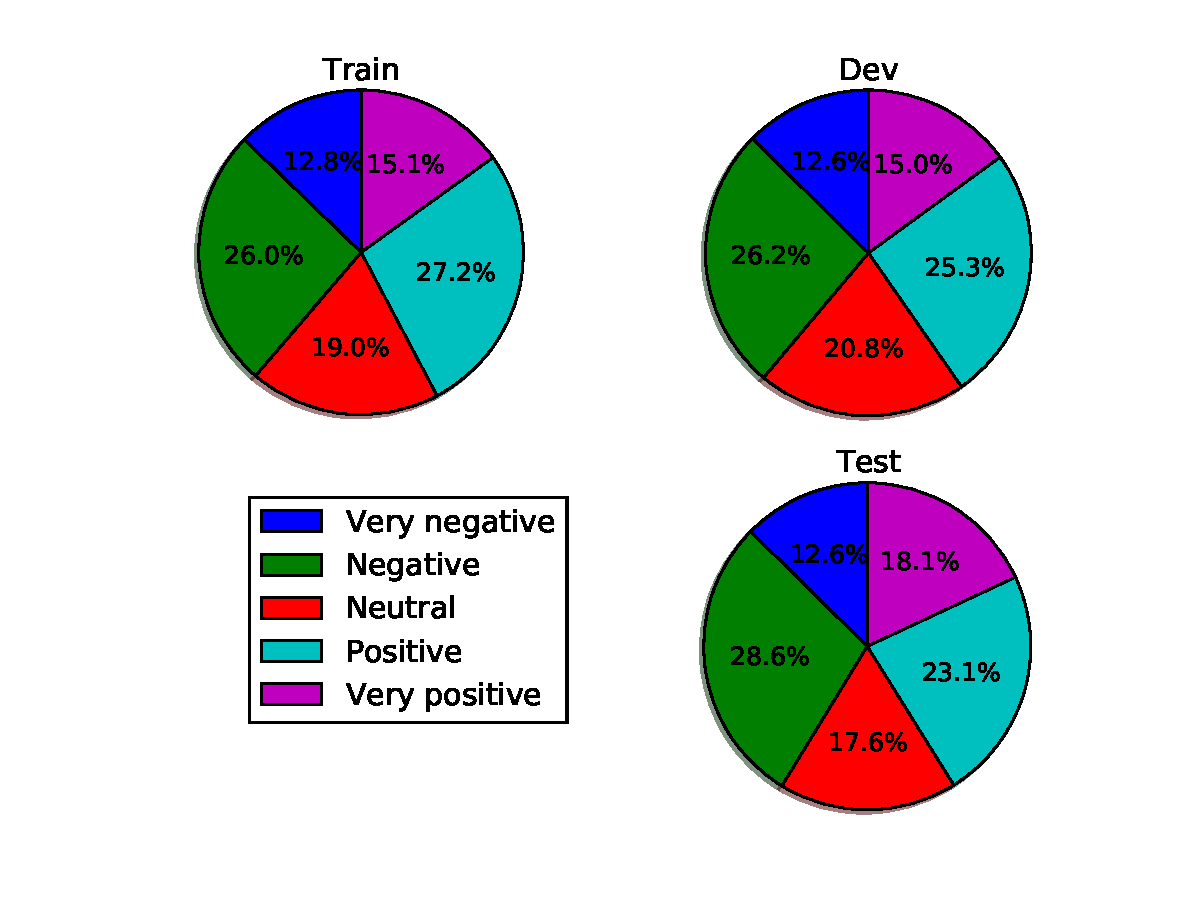
\includegraphics[scale=0.6]{figure/sstfinegrain}
        \caption[SST fine-grain sentiment distribution]{SST fine-grain sentiment distribution}
        \label{fig:sstfinegrain_5}
    \end{minipage}
\end{figure}

\begin{figure}[H]
    \begin{minipage}{\textwidth}
        \centering
        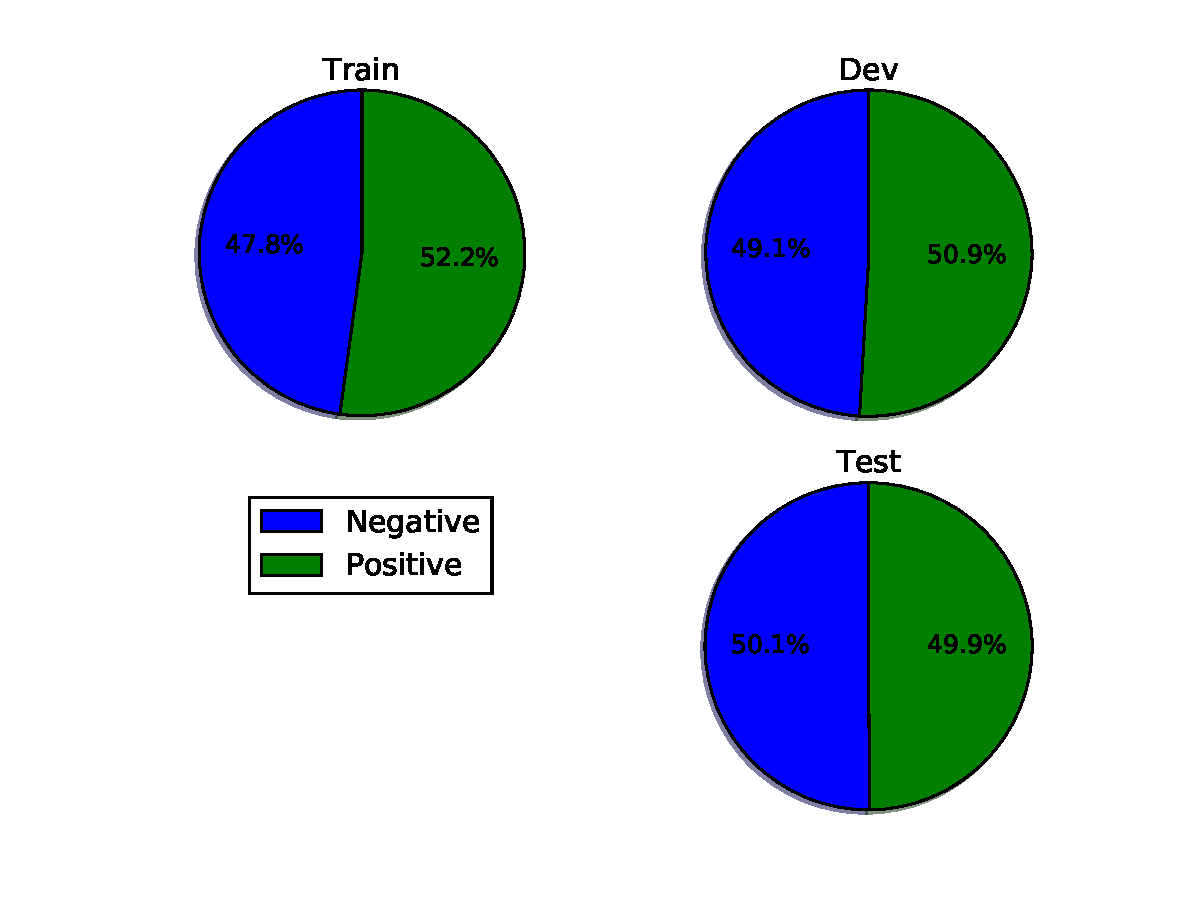
\includegraphics[scale=0.6]{figure/sstbinary}
        \caption[SST binary sentiment distribution]{SST binary sentiment distribution}
        \label{fig:sstbinary_5}
    \end{minipage}
\end{figure}

% Please add the following required packages to your document preamble:
% \usepackage{multirow}
\begin{table}[H]
    \centering
    \caption{SST statistics}
    \label{table:sststatistic_5}
    \begin{tabular}{lllll}
        Number of review       &               &      &                       &  \\ \cline{1-4}
        \multirow{5}{*}{Train} & Very Negative & 1092 & \multirow{2}{*}{3310} &  \\ \cline{2-3}
        & Negative      & 2218 &                       &  \\ \cline{2-4}
        & Neutral       & 1624 &                       &  \\ \cline{2-4}
        & Positive      & 2322 & \multirow{2}{*}{3610} &  \\ \cline{2-3}
        & Very positive & 1288 &                       &  \\ \cline{1-4}
        \multirow{5}{*}{Dev}   & Very Negative & 139  & \multirow{2}{*}{428}  &  \\ \cline{2-3}
        & Negative      & 289  &                       &  \\ \cline{2-4}
        & Neutral       & 229  &                       &  \\ \cline{2-4}
        & Positive      & 279  & \multirow{2}{*}{444}  &  \\ \cline{2-3}
        & Very positive & 165  &                       &  \\ \cline{1-4}
        \multirow{5}{*}{Test}  & Very Negative & 279  & \multirow{2}{*}{912}  &  \\ \cline{2-3}
        & Negative      & 633  &                       &  \\ \cline{2-4}
        & Neutral       & 389  &                       &  \\ \cline{2-4}
        & Positive      & 510  & \multirow{2}{*}{909}  &  \\ \cline{2-3}
        & Very Positive & 399  &                       &  \\ \cline{2-4}
    \end{tabular}
\end{table}
\subsection{Amazon Reviews}
Amazon Reviews (Sec.\ref{sec:amazon}) is a gigantic document-level labeled sentiment dataset.
We only used a small part of this dataset which includes Amazon Movies and TV reviews (7,850,072 reviews)~\cite{mcauley2013hidden}, Amazon Book reviews (22,507,155 reviews) and the new Movies and TV reviews (4,607,047 reviews)~\cite{McAuleyTSH15}~\cite{HeM16}.

\section{Experiment setups}
We index all our experimented models along with their number of parameters in Table.\ref{table:paramtable}.

\begin{table}[H]
    \centering
    \caption{Number of trainable parameters of experimented models}
    \label{table:paramtable}
    \begin{tabular}{lll}
        ~ & Memory Size of RNNs unit & Parameters count \\ \hline
        LSTM                     & 168         & 315,840          \\
        BiLSTM                   & 168         & 315,840          \\
        Constituency Tree-LSTM   & 150         & 316,800          \\
        Dependency Tree-LSTM     & 168         & 315.840          \\
        Constituency TE-Tree-GRU & 150         & 476,103          \\
        Dependency TE-Tree-GRU   & 150         & 316,353          \\
        CNN LSTM                 & 168         & 489,347          \\
        CNN Tree-LSTM            & 150         & 482,153          \\
        2 channel CNN LSTM       & 168         & 729,347          \\
        2 channel CNN Tree-LSTM  & 150         & 722,153
    \end{tabular}
\end{table}
\subsection{Utilizing local syntactic information at each node of Recursive Neural Networks}
\subsubsection{Preprocessing}
\paragraph{Constituency TE-Tree-GRU}
All sentences in Stanford Sentiment Treebank are given in binary constituency parse tree format.
We used CoreNLP~\cite{manning2014stanford} to create non-binary constituency parse tree and annotated Part-of-speech tag (POS-tag) for each node. 
We then used word and tag and tree structure as input for our model.


\paragraph{Dependency TE-Tree-GRU}
We used CoreNLP ~\cite{manning2014stanford} to create dependency parse tree with POS-tags and  Universal Dependencies label between head words and their dependents.


\subsubsection{Hyper-parameters and training}
We initialized our word representations with Glove~\cite{glove} pre-trained word vectors \footnote{Common Crawl (840B tokens, 2.2M vocab, cased, 300d vectors, 2.03 GB download) publicly available at \url{https://nlp.stanford.edu/projects/glove/}}  with default dimension of 300.  We randomly initialize tag and relationship representation (dependency only) vectors of dimension 50. 
We set memory dimensions to 150.

We tuned our model on development dataset using grid search.
Our model was trained using AdaGrad~\cite{duchi2011adaptive} with learning rate of $\{0.1,~ 0.05,~ 0.01\}$ and Adam $\{1e^{-3}, 1e^{-4}\}$, L2 regularization strength of $\{1e^{-3},~ 1e^{-4}, ~ 1e^{-5} \}$, batch size of 25. 
We manually updated our word representation with learning rate $\alpha$ of $\{0.1,~0.05, ~0.01\}$ as Eq.\ref{eq:manuallyupdate}. 
In addition, we used dropout~\cite{krizhevsky2012imagenet} to regularize our model. 
We regularized Tree-GRU with input dropout rate of 0.5 and memory dropout rate at 0.1. 
Sentiment classifier was also regularized with 0.5 dropout rate. 
Tag and rel representation were tuned in the same ways as word representation.

We discovered that training model composition with Adam learning rate of 0.001 and word representation (updated manually) learning rate at 0.05 for 20 epochs yield the best result.
Training more epochs does not improve the performing.

\subsection{Transfer Learning by training word vectors using Glove on Amazon Reviews dataset}
\subsubsection{Hyper-parameters and training}
We use Glove implementation\footnote{Publicly available on Github \url{https://github.com/stanfordnlp/GloVe}} to train word representation.
We set $x_{max} = 100$, vector size to 300, windows size to 20 and the minimum number of word occurrences to be included in the vocabulary to 5.
The training process took the plain text file produced by the \hyperref[sec:preprocessamazonglove]{preprocessing steps} as its input.
In total, the size of the corpus is 4.7 billions tokens.
After the training process, the resulting word embeddings has vocabulary size of 1,734,244.
We named this word embeddings Glove Amazon.
Apart from using Glove Amazon to replace Glove Common Crawl for initializing word embedding layer of Tree-LSTM, the whole training process and hyper-parameters are kept unchanged (Sec.\ref{sec:treelstm}).

\subsection{Combining Recursive Neural Networks with Convolution Neural Networks}
% not yet
% \subsubsection{Preprocessing}
% \paragraph{Steps for preprocessing Amazon dataset for training Language Model}
% \label{sec:preprocessamazonglove-LM}
% \begin{enumerate}
% \item For retraining Glove vectors, we only used new Movies and TV dataset (4,607,047 reviews)~\cite{McAuleyTSH15}~\cite{HeM16}.
% \item All the reviews were grouped by product-ID ("asin" keyword in the \hyperref[sec:amazon]{JSON schema of the dataset}).
% \item In each product-ID group, the reviews were sorted increasingly by their rating ("overall" keyword in the JSON schema of the dataset).
% \item A special character sequence was added at the end of each review to mark its end.
% After that, all the reviews were dumped into a plain text file.
% \item The text file produced from the previous step was tokenized using Stanford Tokenizer~\cite{tokenizerpart}.
% \item The tokenized text file was then divided into training and test set using 95:5 split.
% As this is a pre-training process, we used only 5\% of the data to test if the Language Model was trained properly.
% \end{enumerate}

% Step 2, 3 and 4 are for mitigating the problem of noise in training data which have been presented in Sec.\ref{sec:preprocessamazonglove}.
\subsubsection{Hyper-parameters and training}
For the models with only single input channel, we initialized word representation with Glove vectors~\cite{glove}.
With two word embeddings channels, we initialized one channel using Glove Common Crawl\footnote{\label{glovecommoncrawl}Common Crawl (840B tokens, 2.2M vocabularies, cased, 300d vectors, 2.03 GB download) publicly available at \url{https://nlp.stanford.edu/projects/glove/}} and the other using our Glove Amazon (Sec.\ref{sec:reuse-glove-amazon}).

We tried a variety of convolution filters combination.
For single kernel size, we performed grid search on $\{100, 200, 300\}$ number of kernels of size $\{3, 5\}$.
For two different kernel size, we tried with $\{100, 200\}$ number of kernels for each kernel size.
Output matrices of different kernel sizes were concatenated as if they were with same kernel size.

Our model was trained using AdaGrad~\cite{duchi2011adaptive} with learning rate of $\{0.1,~ 0.05,~ 0.01\}$, L2 regularization of $\{1e^{-3},~ 1e^{-4}, ~ 1e^{-5} \}$, batch size of 25.
We manually update our word representation with learning rate $\alpha$ of $\{0.1,~0.05, ~0.01\}$ following Eq.\ref{eq:manuallyupdate}.
We regularized convolution layer with input dropout rate of 0.5 and output dropout rate of 0.2 in addition to dropout of rate 0.5 at output layer.
We applied the same hyper-parameters grid search for two channels convolution.
\begin{equation}
\label{eq:manuallyupdate}
w = w - \alpha\delta J(\theta)
\end{equation}

We found that 100 filters of size 3 words and 100 filters of size 5 words yield better results compared to single filters size or the number of filters larger than 200. We trained with Adagrad of learning rate of 0.01 and word vectors (updated manually) at learning rate 0.1 give the best result. We trained for 60 epochs for CNN Tree-LSTM and 20 epochs for CNN LSTM. Training 60 epochs on CNN LSTM did not yielded observable better result than 20 epochs.

\section{Experiment results}

% \begin{table}[H]
%     \centering
%     \caption{Experiment result. For our experiment, we report mean accuracies of 5 runs. Max value in bracket.}
%     \label{table:experimentresult}
%     \begin{tabular}{ll}
%         Method                                   & Binary \\ \hline
%         LSTM                                     & 86.40   \\
%         BiLSTM                                   & 85.80   \\ \hline
%         Constituency Tree-LSTM ~\cite{treeLSTM} & 88.00     \\
%         Constituency Tree-LSTM ~\cite{treeLSTM} (Glove Amazon) & 88.85 (89.35) \\
%         Dependency Tree-LSTM  ~\cite{treeLSTM}  & 85.70   \\
%         CNN GRU ~\cite{cnn-rnn}                    & 89.13(89.95) *    \\
%         CNN LSTM ~\cite{cnn-rnn}                    & 89.43(89.56) *    \\ \hline
%         Constituency TE Tree-GRU                 & 87.65 (88.25)  \\
%         Dependency TE Tree-GRU                   & 87.13  (88)  \\ \hline
%         CNN LSTM                                 & 89.10 (89.40)      \\
%         % CNN LSTM (pretrained)**                 &            \\
%         2 Channel CNN LSTM                        & 89.54    (89.79)    \\
%         % 2 Channel CNN LSTM (pretrained)**        &         \\
%         CNN Tree-LSTM                            & 88.82 (88.92) \\
%         CNN Tree-LSTM (Glove Amazon)             & 88.96 (89.18) \\
%         2 Channel CNN Tree-LSTM                  & 89.66 (90.12)
%     \end{tabular}
% \end{table}

\begin{table}[H]
    \centering
    \caption[Experiment result on SST]{Experiment results of models evaluated on Stanford Sentiment Treebank with binary setting.
The models which have both data of mean(std) and max are models which have been evaluated by us.
For these models, we report mean, standard deviation and max of 5 runs.
If a model has data of only mean(std) or only max, the data was taken from its originated research paper.
If the data of both mean(std) and max is missing, the model was not evaluated yet.
\textit{(*): Result reported by the original paper.}}
    \label{table:experimentresult}
    \begin{tabular}{c|lll}
    \textbf{Block}    & \textbf{Model}  & \textbf{Mean(std)} & \textbf{Max}   \\
\Xhline{3\arrayrulewidth}
\Xhline{3\arrayrulewidth}

    \multirow{4}{*}{A} & CNN-non-static~\cite{KimCNN} & - & 87.20\Tstrut \\
        & CNN-multichannel~\cite{KimCNN} & - & 88.10 \\
    & DCNN~\cite{DCNN} & - & 86.80 \\
    & MVCNN~\cite{2-layer-cnn} & - & 89.40 \\
\hline
        \multirow{5}{*}{B} & LSTM~\cite{originLSTM}    & 86.64 (0.27) & 86.93  \\
        & BiLSTM~\cite{GravesLSTM}  & 85.80 (0.69) & 86.43   \\
        & 2-layer LSTM~\cite{GravesLSTM} & 86.30 (0.60) & - \\
         & 2-layer Bidirectional LSTM~\cite{GravesLSTM} & 87.20 (1.00) & - \\
         & DMN~\cite{attention-gru} & - & 88.60 \\
\hline
        \multirow{5}{*}{C} & RNTN~\cite{socher2013recursive}  & - & 85.40  \\
        & DRNN~\cite{IrsoyDRNN} & - & 86.60 \\
        & TE-RNTN~\cite{tag-embedding-rnn} & - & 87.70 \\
        & Dependency Tree-LSTM  ~\cite{treeLSTM}  & 85.70 (0.30)  & 85.80 \\
         & Constituency Tree-LSTM ~\cite{treeLSTM} & 88.00 (0.40)    &   88.19\\
\hline
        \multirow{3}{*}{D} & GICF~\cite{group-instance} & - & 85.70 \\
         & Paragraph-Vec~\cite{ParagraphVec} & - & 87.80 \\
         & LSTM (PARAGRAM-SL999)~\cite{wieting2015towards} & 87.98 (0.46) & 88.50 (89.20)*
          \\
\hline
         \multirow{2}{*}{E}  & CNN GRU ~\cite{cnn-rnn}                    & 89.13 (0.29)  &  89.61 (89.95)*    \\
         & CNN LSTM ~\cite{cnn-rnn}                    & 89.43 (0.28)  & 89.72 (89.56)*\Bstrut    \\
\Xhline{3\arrayrulewidth}
\Xhline{3\arrayrulewidth}
         \multirow{2}{*}{F} & Constituency TE Tree-GRU                 & 87.65 (0.34) & 88.25\Tstrut \\
          & Dependency TE Tree-GRU                   & 87.13 (0.70)  & 88.00\Bstrut \\
\hline
\hline
        \multirow{1}{*}{G} & Constituency Tree-LSTM ~\cite{treeLSTM} (Glove Amazon) & 88.85 (0.44) & 89.35\Tstrut\Bstrut \\
\hline
\hline
        \multirow{3}{*}{H} & CNN LSTM                                 & 89.10 (0.39)  & 89.40 \Tstrut  \\
        & 2 Channel CNN LSTM                        & 89.54    (0.22) & 89.79    \\
        & Multichannel CNN LSTM (pretrained) & - & - \\
\hline
        \multirow{4}{*}{I} & CNN Tree-LSTM                            & 88.82 (0.13) & 88.92 \\
        & CNN Tree-LSTM (Glove Amazon)             & 88.96 (0.24) & 89.18 \\
        & 2 Channel CNN Tree-LSTM  &\textbf{89.69 (0.36)} & \textbf{90.12}    \\
        & Multichannel CNN Tree-LSTM (pretrained)        & - & -        \\
    \end{tabular}
\end{table}


% \textit{(***): CNN and LSTM layer are initialize using pre-trained parameters from Section \ref{sec:CNNtree}}

Experiment results are summaries in Table \ref{table:experimentresult}.
Table \ref{table:experimentresult} is divided into two parts.
The first part is from Block A to E, which contains all baselines model.
The second part is from Block F to I, which contains all models which were proposed and evaluated by us.

\textbf{Descriptions of each Block in the first part}:
\begin{description}
\item[Block A] contains Multilayer Convolution Neural Networks models.
CNN-non-static and CNN-multichannel~\cite{KimCNN} are single layer CNN (Sec.\ref{kim-cnn}).
DCNN~\cite{DCNN} and MVCNN~\cite{2-layer-cnn} are multilayer CNN, with MVCNN is a very large model  which has 2 layers, 5 word embeddings channels and unsupervised pre-train using the method of Sentence Encoding (Sec.\ref{sec:2-layer-cnn})
\item[Block B] contains sequential/recurrent models.
 LSTM~\cite{originLSTM}, BiLSTM~\cite{GravesLSTM}, 2-layer LSTM~\cite{GravesLSTM} and 2-layer Bidirectional LSTM~\cite{GravesLSTM} have been described in Sec.\ref{sec:RNN}.
DMN~\cite{attention-gru} is a sophisticated model used GRU with attention mechanism and episodic memory.
\item[Block C] contains models which belong to the family of Recursive Neural Networks (tree-structured model).
RNTN~\cite{socher2013recursive} is the first recursive neural network to successfully apply on sentence-level sentiment analysis (Stanford Sentiment Treebank).
It was inspired by the idea that natural languages have recursive structure, to understand a sentence we must understand its phrases and, to understand a phrase, we must understand its words.
DRNN~\cite{IrsoyDRNN} is a multilayered extension of RNTN.
TE-RNTN is also an extension of RNTN which utilize the local syntactic information at each node of a sentence's parse tree.
Dependency and Constituency Tree-LSTM~\cite{treeLSTM} are tree-structured versions of LSTM which have been described in Sec.\ref{sec:treelstm}.

\item[Block D] contains transfer learning methods, which utilized a large amount of data other than Stanford Sentiment Treebank.
GICF~\cite{group-instance} is an attempt to learn to classify sentiments of sentences (in Stanford Sentiment Treebank) from training dataset which contains only document-level sentiment labels.
Paragraph-Vec~\cite{ParagraphVec} is a method that learns to encode any sequence of words into a vector with the purpose of maximizing the likelihood of words which appear in that sequence given the encoding vector.
LSTM (PARAGRAM-SL999)~\cite{wieting2015towards} is a LSTM models with word embeddings layer initialized by PARAGRAM-SL999, word vectors trained on a large paraphrase dataset (PPDB~\cite{ganitkevitch2013ppdb}) % which was trained using a large paraphrase dataset (PPDB~\cite{ganitkevitch2013ppdb}).
In our experiments with LSTM (PARAGRAM-SL999), we used the implementation and pre-trained word vectors which are publicly available on the author website\footnote{\url{http://ttic.uchicago.edu/~wieting/}}.

\item[Block E] contains models which combine Convolution Neural Networks and Recurrent Neural Networks.
CNN GRU and CNN LSTM~\cite{cnn-rnn} have been described in detail in Sec.\ref{cnn-rnn}.
In our experiments with CNN GRU and CNN LSTM, we used the implementation publicly published by the authors\footnote{\url{https://github.com/ultimate010/crnn}}.
\end{description}

\textbf{Descriptions of each Block in the second part}:
\begin{description}
\item[Block F] contains models which follow our approach of utilizing local syntactic information at each node of Recursive Neural Networks (Sec.\ref{sec:VTtree})
\item[Block G] contains the experiment which follows our approach of applying Transfer Learning by retraining Glove on Amazon Reviews dataset (Sec.\ref{sec:gloveamazone})
\item[Block H and I] contain the models which follow our approach of combining Recursive Neural Networks with Convolution Neural Networks (Sec.\ref{sec:CNNtree}).
Block H is for sequential architects, while Block I is for tree-structured architects.
\end{description}
\section{Discussions}
\subsection{Utilizing local syntactic information at each node of Recursive Neural Networks}
Our dependency TE Tree-GRU outperformed Dependency Tree-LSTM when using the same dependency parsed dataset.
But disappointedly, TE Tree-GRU underperformed Dependency Tree-LSTM on Semantic Relatedness task (SemEval 2014, Task 1~\cite{SemeEvalTask1}) which pointed out the strength of Dependency Tree-LSTM and the main reason why it was presented in the original paper~\cite{treeLSTM}.
Constituency TE Tree-GRU model is slightly better than Dependency TE Tree-GRU.
This performance gap is expected because Dependency parse tree has less labeled node comparing to Constituency parse tree~\cite{treeLSTM}.

\label{unproved:tag-useless}
On overall, this approach does not improving Tree-LSTMs, it might be because Tree-LSTMs have already utilized the information in word embeddings and the local syntactic information from tag embeddings added no more value.


\subsection{Transfer Learning by retraining Glove on Amazon Reviews dataset}
\label{fact:glove-amazon-improve-tree}
In Block G, Constituency Tree-LSTM using Glove Amazon largely outperformed Constituency Tree-LSTM using Glove Common Crawl even though it was trained on significantly larger dataset (840B tokens) compared to our preprocessed Amazon Reviews (4.7B tokens) (Sec.\ref{sec:gloveamazone}).
This method also outperformed all the Transfer Learning methods in Block D.
Compared to Glove Amazon method, originally,  Paragraph-Vec~\cite{ParagraphVec} cannot be fine-tuning in a supervised manner.
We also used PARAGRAM-SL999 for initializing the word embeddings layer of Constituency Tree-LSTM,
the results (of 8 runs with mean 87.175\% and standard deviation 0.69) were not as good as those of Glove Common Crawl.

These results support our hypothesis that by training word embeddings on review documents, especially movie or book reviews, we can capture more rare words and also the different way people use words (or different word relationships) when they express their opinions on movies or books (Sec.\ref{movie-hypothesis}).

\subsection{Combining Recursive Neural Networks with Convolution Neural Networks}
\label{proved:tree-conv-benefit}
The fact that CNN Tree-LSTM outperforms Constituency Tree-LSTM~\cite{treeLSTM} supports our hypothesis on the benefits of combining convolution layers with Tree-LSTM (Sec.\ref{conv-tree-benefits}).
Due to using similar architects, CNN LSTM was comparable with CNN GRU and CNN LSTM~\cite{cnn-rnn}. \label{unproved:cnn-treelstm-overfit}
CNN Tree-LSTM performed worst than CNN LSTM, the reason might because of over-fitting.
We will prove this hypothesis by looking at the plots of error rate on training and validation set of these two models.

\label{proved:Amazon-adv-Common}
We have seen that Glove Amazon improved Tree-LSTM in Sec.\ref{fact:glove-amazon-improve-tree}.
In these experiments (Block I), Glove Amazon also improved CNN Tree-LSTM.
We can conclude that Amazon Glove captured some good\footnote{good for the task of sentiment analysis of movie reviews} features that does not exist or hardly be extracted in Glove Common Crawl.

According to Table.\ref{table:paramtable}, the number of parameters of 2 Channel CNN Tree-LSTM (722,153) is much larger than that of CNN Tree-LSTM (482,153), which makes it more likely for 2 Channel CNN Tree-LSTM to over-fit the training data.
However, in fact, 2 Channel CNN Tree-LSTM was able to archive much higher accuracy than both CNN Tree-LSTM (Glove Amazon) and CNN Tree-LSTM (Glove Common Crawl).\label{proved:Common-syn-Amazon}
The result proves that there are some features only appearing in Glove Common Crawl or when combining both Glove Amazon and Glove Common Crawl.
Otherwise, there would not be any improvement.

At the time of this submission\footnote{20/07/2017}, we have not finished our experiments on unsupervised pre-training methods (Sec.\ref{enhan-unsupervised-pretrain}), we will add the results of these experiments as soon as possible.

